\documentclass[11pt]{amsbook}
\usepackage{../HBSuerDemir}
\usepackage{wrapfig}

\begin{document}

% ++++++++++++++++++++++++++++++++++++++
\hPage{b1p2/353}
% ++++++++++++++++++++++++++++++++++++++

	\begin{hEnumerateArabic}
		\item
		$ 
		\int_{a}^{b} \! f(x) \, \hDif x
		\leq
		\int_{a}^{b} \! g(x) \, \hDif x
		\quad \text{if} \quad
		f(x) \leq g(x)
		$

		\item
		$
		\int_{a}^{b} \! f(x) \, \hDif x
		\quad \text{is the area bounded by the curves of} \quad
		y = f(x), y = 0
		\quad \text{and} \hNewLine
		x = a, x = b
		\quad \text{if} \quad
		f(x) > 0
		\quad \text{on} \quad
		(a,b)
		$
	\end{hEnumerateArabic}


\begin{exmp}
\label{exmp:b1p2_353_firstExample} 
	Find the volume of the solid with circular base of radius 5 m,
	and each cross section perpendicular to a definite diameter is a square.
	
	\begin{hSolution}
		Let us take the definite diameter as
		$ x $-axis
		and the one perpendicular to it as 
		$ y $-axis.
		Then the equation of the circle is
		$ x^{2} + y^{2} = 25 $.
		From the symmetry of the solid with respect to the cross section through y-axis
		the volume
		$ V $
		will be twice as that for
		$ 0 \leq x \leq 5 $
		.

		\begin{figure}[h]
		  \begin{center}
		    \includegraphics[scale=0.4]{images/b1p2-353-fig01.png}
		  \end{center}
		  \caption{Circular base and some square cross sections of the solid in Example \ref{exmp:b1p2_353_firstExample}}
		\end{figure}

		For a regular partition of
		$ (0; 5) $
		we have congruent subintervals of lengths
		$ 5/n $.
		The area of the cross section through the point
		$ (x_{k}, y_{k}) $
		being
		$ (2y_{k})^{2} $
		the volume
		$ V_{k} $
		of the slice with thickness
		$ 5/n $
		is
		$ 4y_{k}^{2} \cdot 5/n $:

		\begin{equation}
			V_{k} 
			= \frac{20}{n} y_{k}^{2} 
			= \frac{20}{n} (25 - x_{k}^{2}) 
			= \frac{20}{n} ( 25 - \left( k \frac{5}{n} \right) ^{2} ) 
			= \frac{500}{n} \left( 1 - \frac{ k^{2} }{ n^{2} } \right)
		\end{equation}

		\begin{equation}
			\begin{split}
			\sum_{k=1}^{n} V_{k}
			& = \frac{500}{n} \sum_{k=1}^{n} \left( 1 - \frac{ k^{2} }{ n^{2} } \right) 
			  = \frac{500}{n} \left( n - \frac{ \sum k^{2} }{ n^{2} } \right)
			  \hNewLine
			& = 500 \left( 1 - \frac{n(n + 1)(2n + 1)}{6n^{3}} \right)
			\end{split}
		\end{equation}

		\begin{equation}
			\begin{split}
			v
			& = 2 \lim_{n \to \infty} \sum_{k=1}^{n} V_{k} 
			= 1000 \left( 1 - lim \frac{ n(n + 1)(2n + 1) }{ 6n^{3} } \right)
			\hNewLine
			& = 1000 \left( 1 - \frac{1}{3} \right) = ( 2000/3 ) m^{3}.
			\end{split}
		\end{equation}
	\end{hSolution}
\end{exmp}


\end{document}
